\documentclass[11pt]{article}
\usepackage[margin=1in]{geometry}
\usepackage{graphicx}
\usepackage{hyperref}
\usepackage{xcolor}
\usepackage{parskip}
\usepackage{enumitem}
\usepackage{booktabs}
\usepackage{fancyvrb}

\definecolor{teal}{HTML}{0D9488}
\definecolor{darkbg}{HTML}{1A1A2E}

\hypersetup{
  colorlinks=true,
  linkcolor=teal!80!black,
  urlcolor=teal!80!black
}

\title{\textcolor{teal}{\Huge Curious Jack}\\[6pt]
\large A User Guide}
\author{Paul Fishwick and Claude Code}
\date{February 2026}

\begin{document}
\maketitle

\tableofcontents
\newpage

% -----------------------------------------------------------------------
\section{Introduction}
% -----------------------------------------------------------------------

Curiosity is a web application that uses multiple AI models to answer
questions about an image. A user uploads a photograph or artwork, selects
educational parameters, and types one or more questions. The application
sends each question --- together with the image --- to three large language
models (Google Gemini, OpenAI GPT, and Anthropic Claude) running in
parallel via the OpenRouter API. A coordinator model then synthesizes the
three responses into a single, level-appropriate answer and aligns it to
the relevant educational standards for the chosen US state.

% -----------------------------------------------------------------------
\section{Getting Started}
% -----------------------------------------------------------------------

\subsection{Starting the Server}

Curiosity runs as a local Node.js server. From the project directory, run
the included start script:

\begin{Verbatim}[fontsize=\small]
./start
\end{Verbatim}

The server starts on \texttt{http://localhost:3456}. Open that URL in your
browser to use the application.

To stop the server, run:

\begin{Verbatim}[fontsize=\small]
./stop
\end{Verbatim}

% -----------------------------------------------------------------------
\section{API Key Configuration}
% -----------------------------------------------------------------------

Curiosity requires an \href{https://openrouter.ai}{OpenRouter} API key to
call the language models. There are two ways to provide it.

\subsection{Environment Variable (Recommended)}

Set \texttt{OPENROUTER\_API\_KEY} in your terminal before starting the
server, or add it permanently to \texttt{\textasciitilde/.env}:

\begin{Verbatim}[fontsize=\small]
# Temporary (current terminal session only)
export OPENROUTER_API_KEY=sk-or-...
./start

# Permanent (add to ~/.env)
OPENROUTER_API_KEY=sk-or-...
\end{Verbatim}

When the key is found at startup, the application skips the modal entirely
and the key never touches the browser or local storage --- the most secure
option.

\subsection{In-Browser Modal}

If no environment variable is set, the application checks the browser's
\texttt{localStorage} for a previously saved key. If none is found, the
API Key modal appears, as shown in Figure~\ref{fig:modal}. Enter your
OpenRouter key and click \textsf{Save \& Continue}. The key is saved to
\texttt{localStorage} so it persists across page reloads.

\begin{figure}[h]
\centering
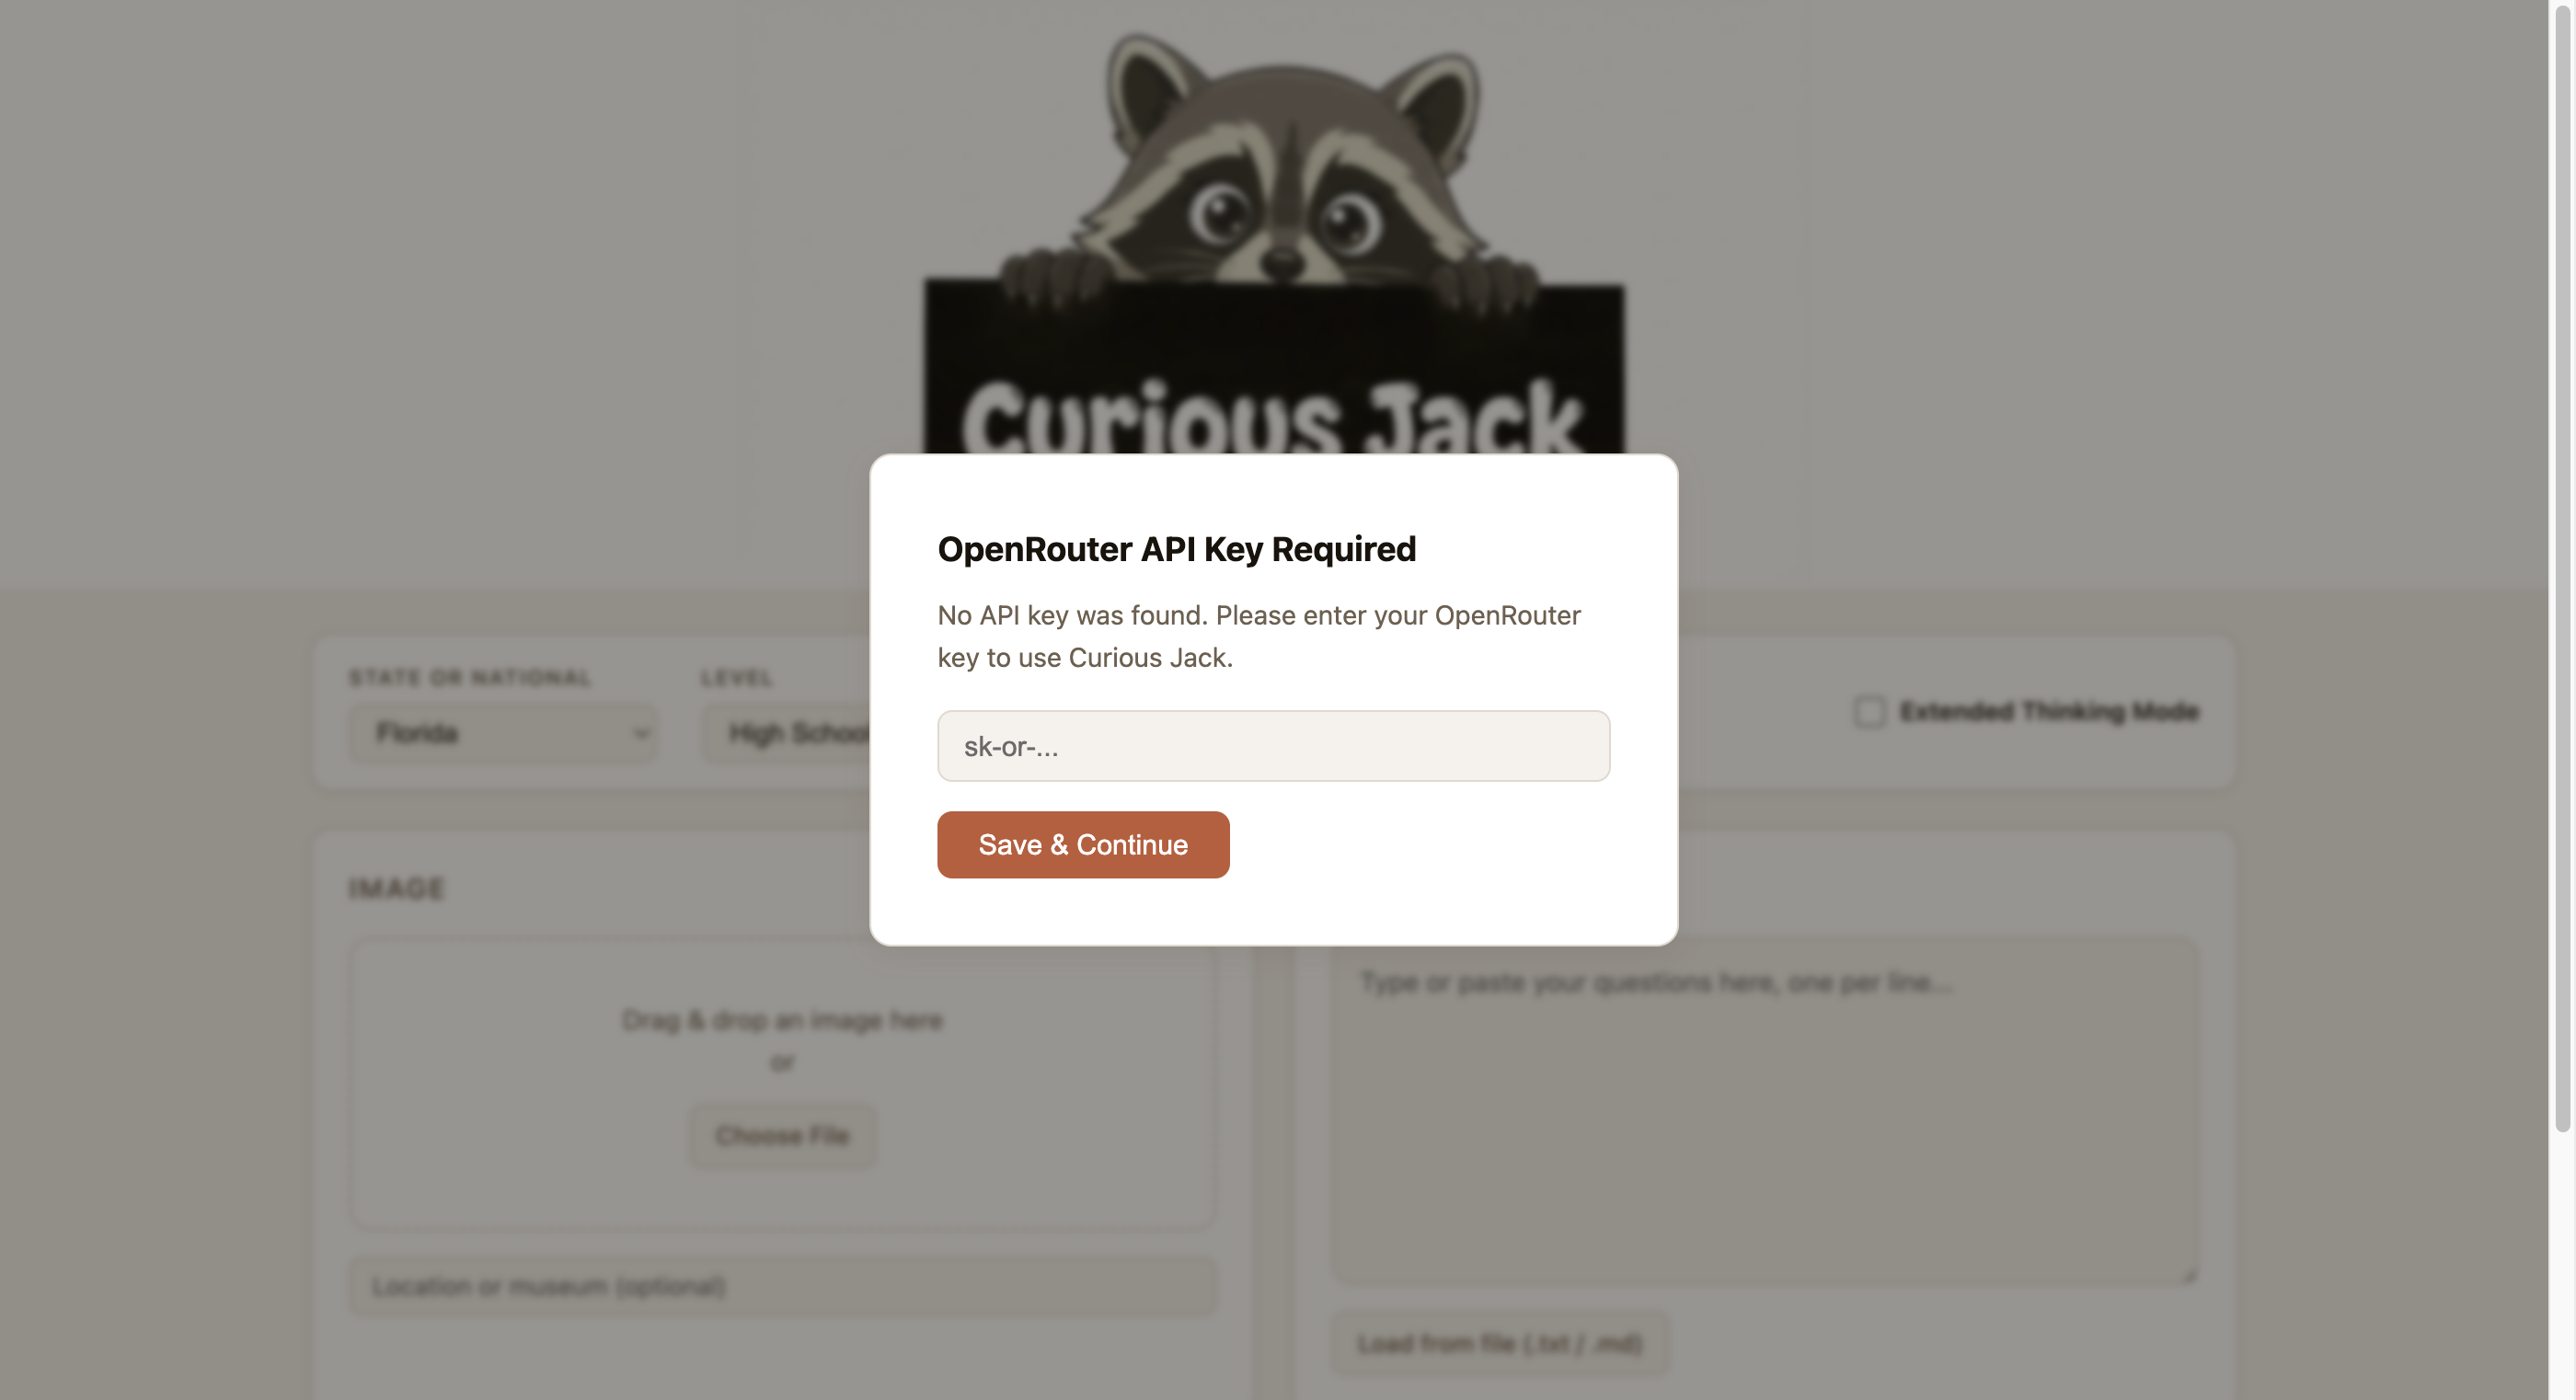
\includegraphics[width=0.75\textwidth]{modal.png}
\caption{The API key modal appears on first use when no server-side key
is configured. The key is stored in \texttt{localStorage} for subsequent
visits.}
\label{fig:modal}
\end{figure}

% -----------------------------------------------------------------------
\section{The Interface}
% -----------------------------------------------------------------------

The main interface, shown in Figure~\ref{fig:main}, consists of a
parameters bar at the top and two input cards below it --- one for the
image and one for the questions.

\begin{figure}[h]
\centering
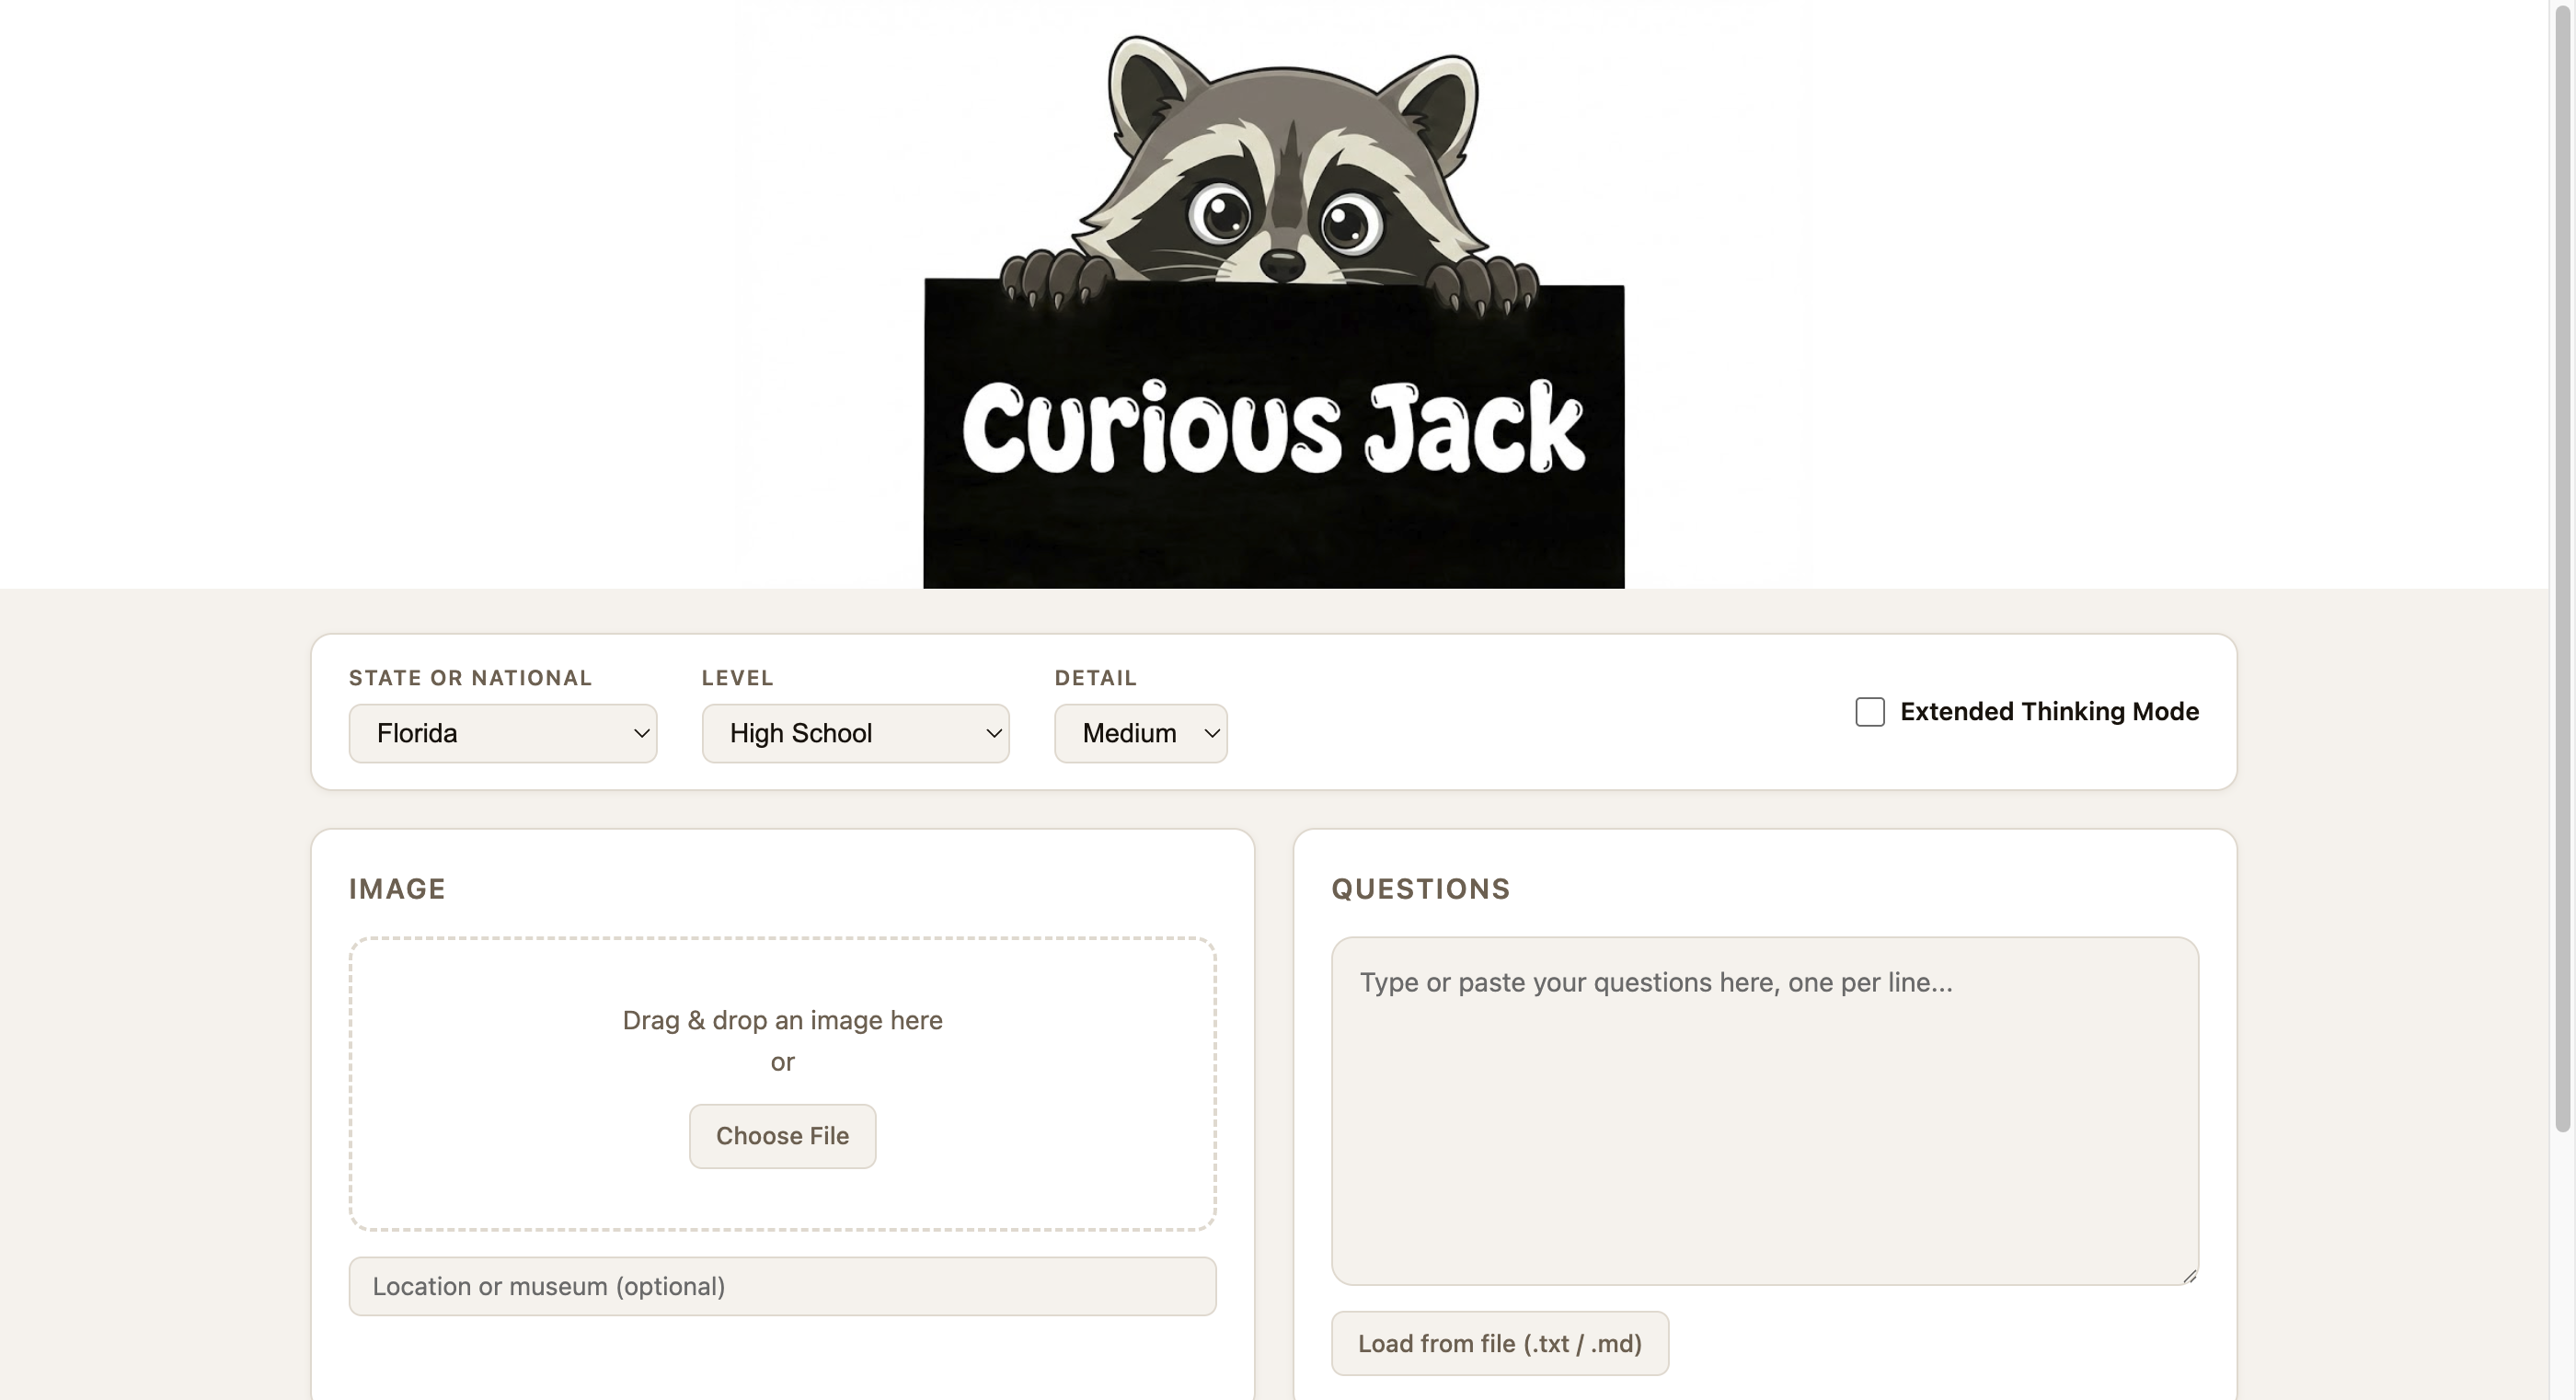
\includegraphics[width=0.95\textwidth]{main.png}
\caption{The main Curiosity interface. The parameters bar runs across the
top; the image upload card is on the left and the questions card is on
the right.}
\label{fig:main}
\end{figure}

\subsection{Parameters Bar}

Four parameters shape the AI response:

\begin{itemize}[nosep]
  \item \textbf{State} --- the US state whose educational standards are
        cited in the results (e.g.\ Florida, Texas, National).
  \item \textbf{Level} --- the academic level of the answer: Elementary,
        Middle, High School, or Advanced / College.
  \item \textbf{Detail} --- Low (one subject, concise), Medium (two or
        three subjects), or High (four or more subjects, comprehensive).
  \item \textbf{Extended Thinking Mode} --- when checked, each model uses
        its extended reasoning capability (Claude uses \texttt{thinking}
        blocks, Gemini uses the \texttt{:thinking} variant, GPT uses
        \texttt{reasoning\_effort: high}).
\end{itemize}

\subsection{Uploading an Image}

Drag and drop an image onto the left card or click \textsf{Choose File}
to open a file picker. Once loaded, a preview of the image replaces the
drop zone. An optional \textsf{Location or museum} field lets you note
where the image was taken or sourced; this context is passed to the
models and included in the exported report.

\subsection{Entering Questions}

Type one question per line in the right card. You may also click
\textsf{Load from file} to populate the textarea from a \texttt{.txt} or
\texttt{.md} file. Blank lines and Markdown headers are ignored, so you
can paste a structured notes file directly. Figure~\ref{fig:ready} shows
the application with an image loaded and questions ready.

\begin{figure}[h]
\centering
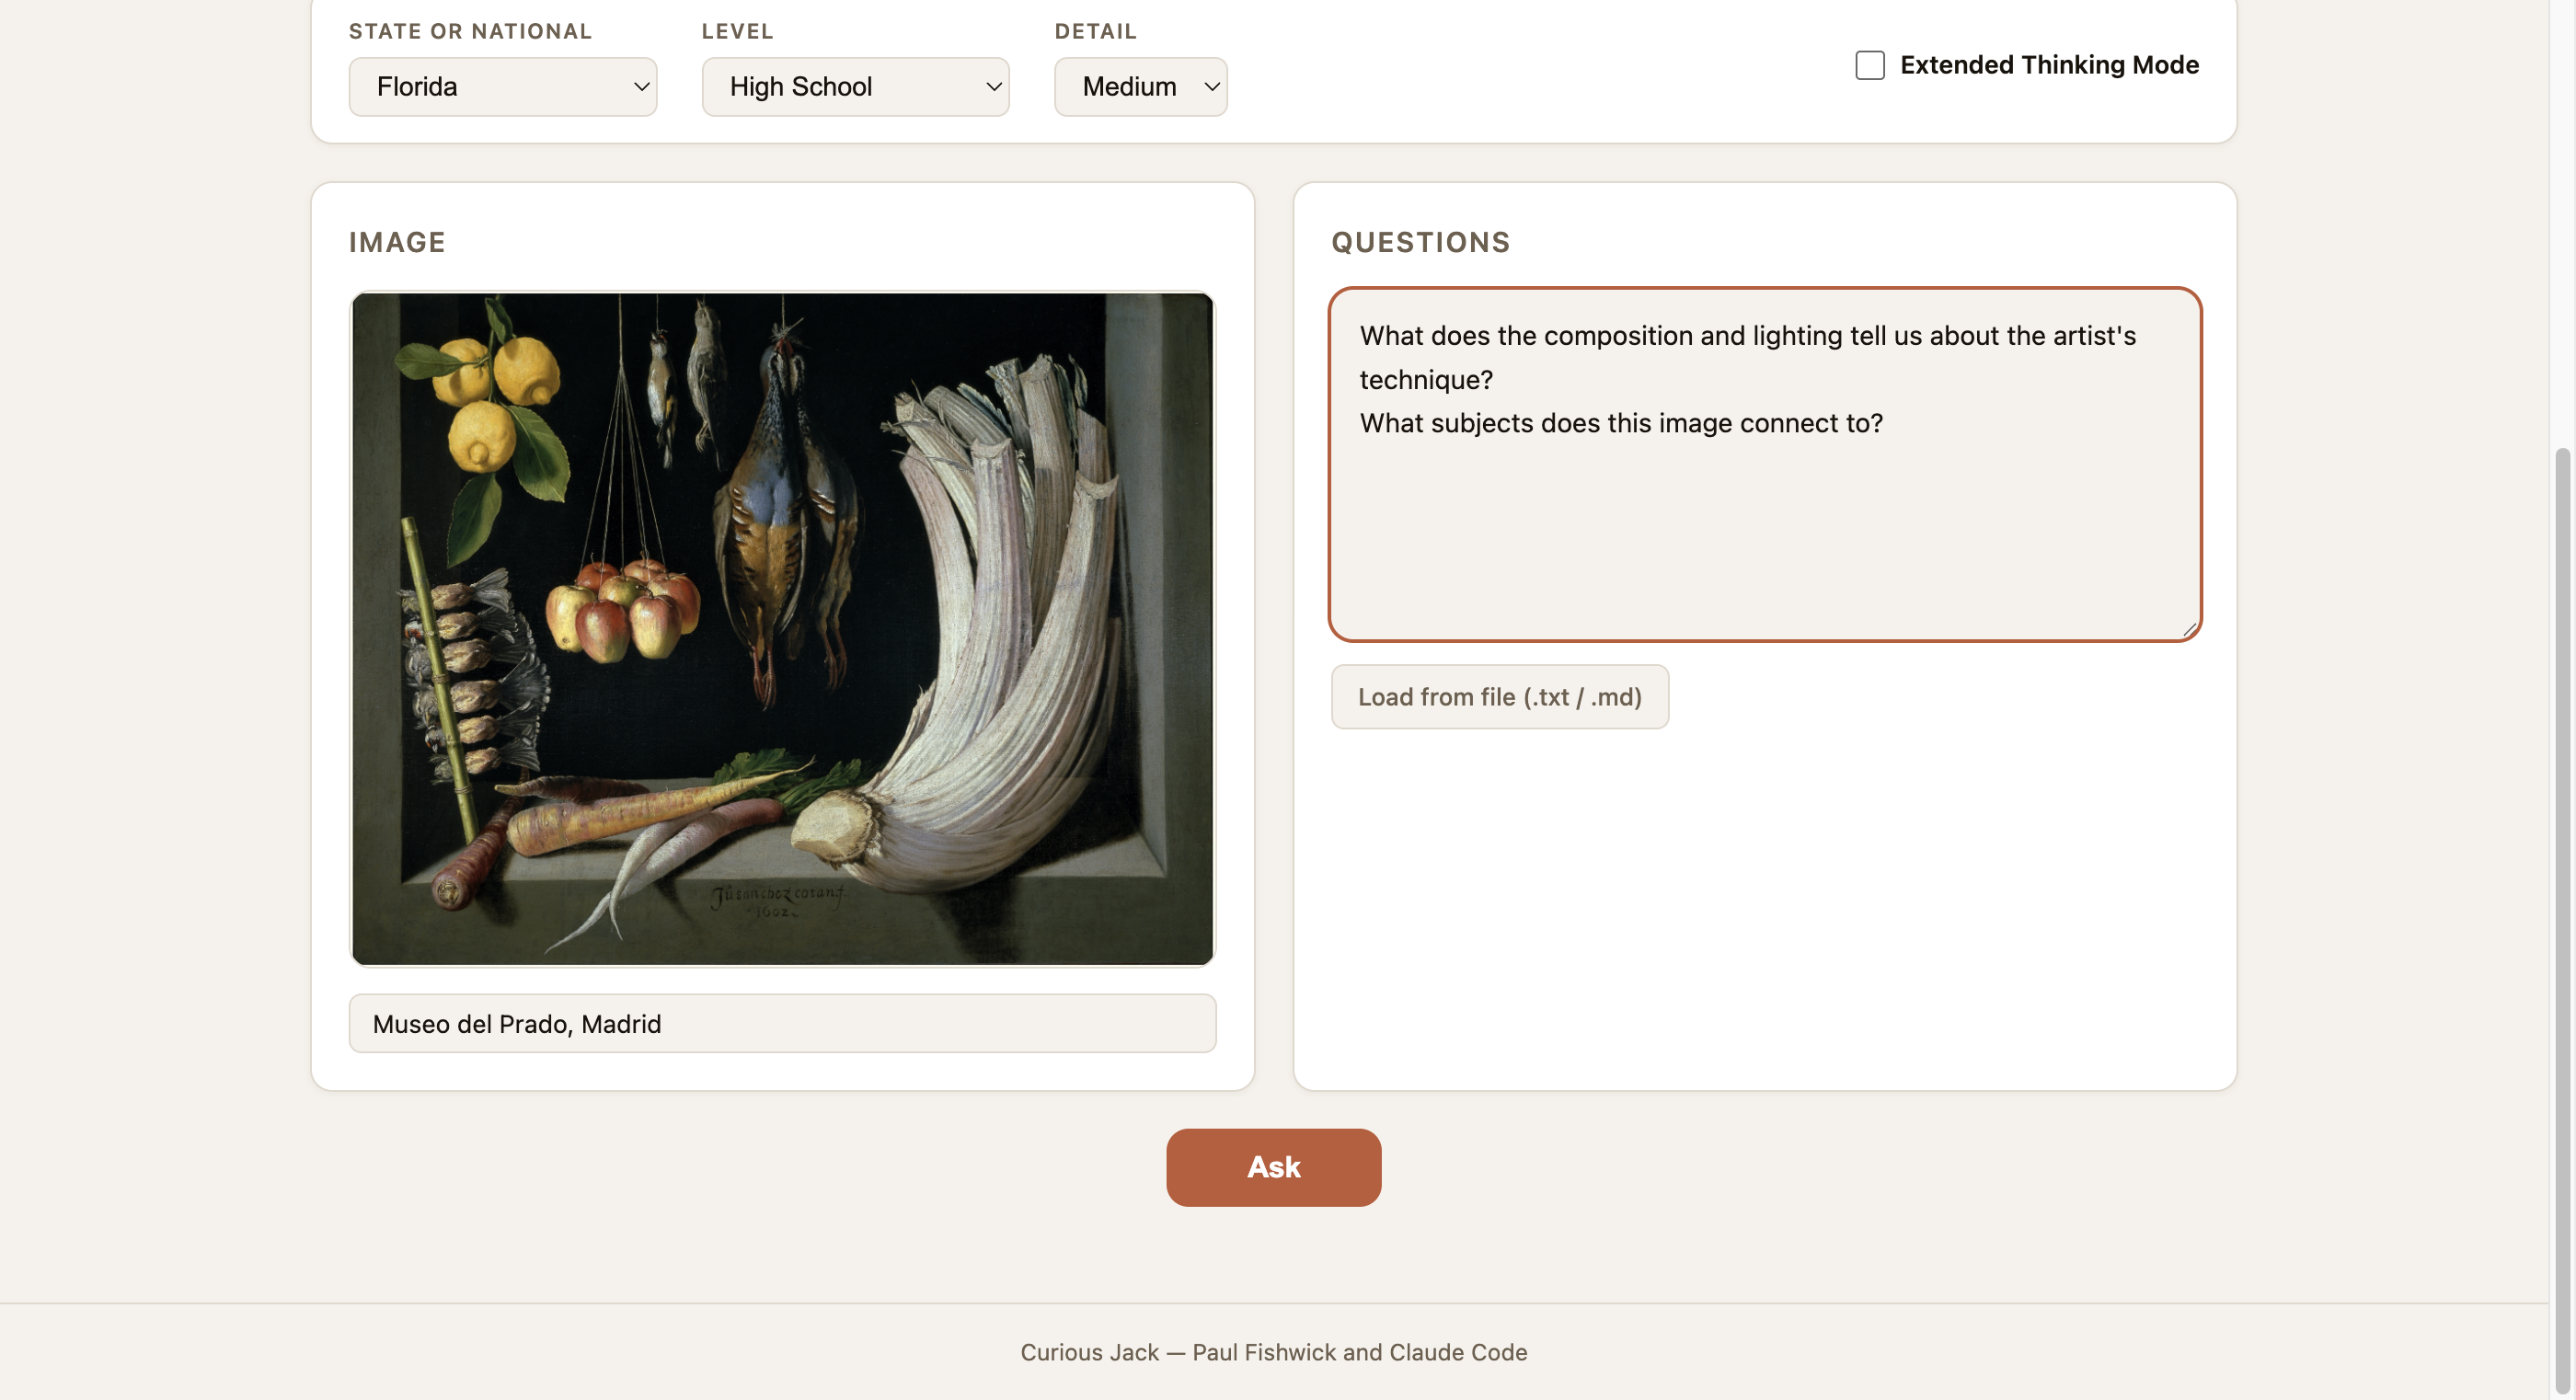
\includegraphics[width=0.95\textwidth]{ready.png}
\caption{The application with an image uploaded and questions entered,
ready to submit. The image preview replaces the drop zone and a location
note has been added.}
\label{fig:ready}
\end{figure}

% -----------------------------------------------------------------------
\section{Results}
% -----------------------------------------------------------------------

Clicking \textsf{Ask} processes each question in turn. A progress bar and
label track the current question number. As each question completes, its
answer card appears and scrolls into view. A sample results card is shown
in Figure~\ref{fig:results}.

Each card contains:

\begin{itemize}[nosep]
  \item The question number and the original question text.
  \item \textbf{Subject tags} --- the academic disciplines identified by
        the coordinator model (e.g.\ Art History, Physics, Chemistry).
  \item \textbf{Answer} --- a synthesized, markdown-formatted explanation
        that notes where the three worker models agreed and where they
        differed.
  \item \textbf{Educational Standards} --- one to three standards from
        the chosen state that are directly relevant to the question,
        with standard codes and links to the official standards pages.
\end{itemize}

\begin{figure}[h]
\centering
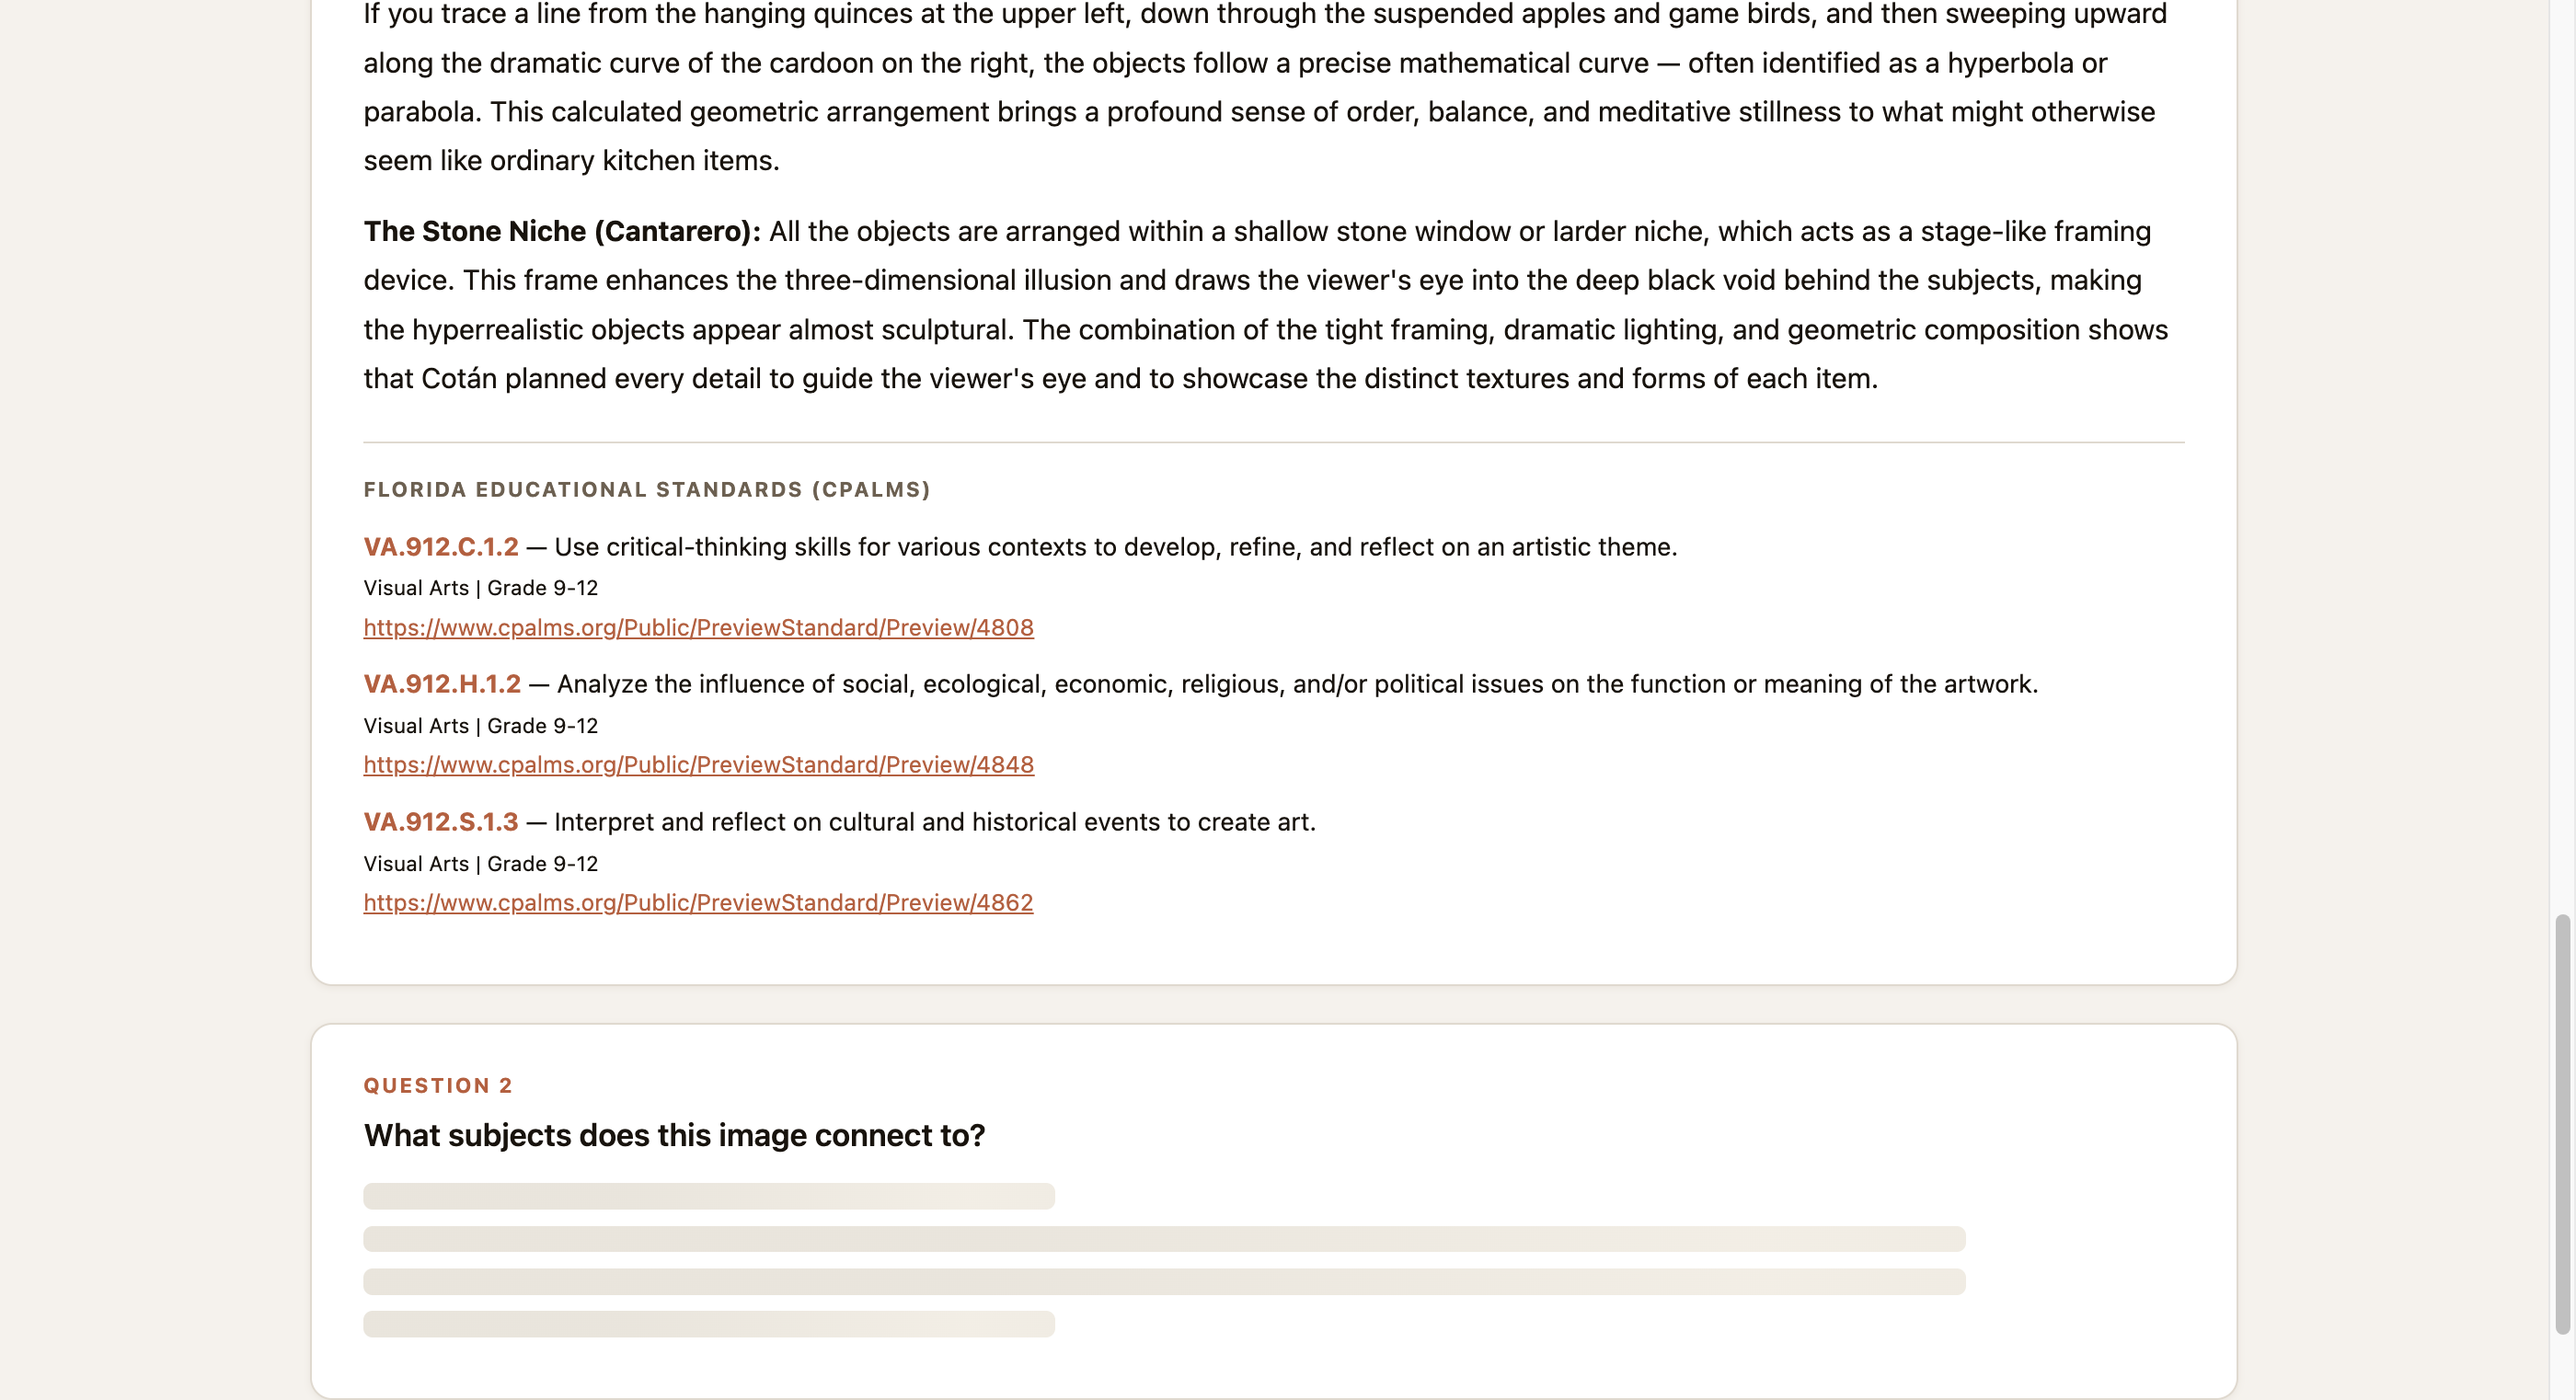
\includegraphics[width=0.95\textwidth]{results.png}
\caption{A completed answer card showing subject tags, the synthesized
answer, and aligned Florida educational standards with CPALMS codes and
links.}
\label{fig:results}
\end{figure}

\subsection{Multi-Model Synthesis}

Internally, each question is sent to three worker models in parallel:

\begin{table}[h]
\centering
\begin{tabular}{ll}
\toprule
\textbf{Worker} & \textbf{Model (via OpenRouter)} \\
\midrule
Gemini  & \texttt{google/gemini-3.1-pro-preview} \\
OpenAI  & \texttt{openai/gpt-5.2} \\
Claude  & \texttt{anthropic/claude-opus-4-6} \\
\midrule
Coordinator & \texttt{anthropic/claude-opus-4-6} \\
\bottomrule
\end{tabular}
\caption{The four model roles used per question. The coordinator
synthesizes the three worker responses.}
\label{tab:models}
\end{table}

The coordinator is instructed to: state majority-agreed facts
confidently, acknowledge genuine disagreements, incorporate unique
insights from individual workers where plausible, and align the final
answer to the chosen educational standards.

\subsection{Image Generation}

If a question asks the AI to \emph{create} or \emph{generate} an image
(e.g.\ ``Draw a diagram of\ldots''), the coordinator routes the request
to Google Gemini's image generation model (\texttt{gemini-3-pro-image-preview})
rather than returning a text answer. The generated image is displayed in
the results card with a download link.

% -----------------------------------------------------------------------
\section{Export}
% -----------------------------------------------------------------------

After all questions are answered, two export buttons appear below the
results:

\begin{itemize}[nosep]
  \item \textsf{Export Markdown} --- downloads a \texttt{.md} file
        containing the full report: parameters, subject image (embedded
        as base64), all questions, answers, and standards.
  \item \textsf{Export PDF} --- opens the browser's print dialog. The
        print stylesheet hides all controls and displays only the banner,
        parameters, image, and answer cards, producing a clean PDF.
\end{itemize}

Sessions are also auto-saved to the server under
\texttt{images/<label>/session.json} (alongside a copy of the image),
where \texttt{<label>} is a short descriptive name generated by the
coordinator model from the uploaded image.

% -----------------------------------------------------------------------
\section{Security}
% -----------------------------------------------------------------------

Because the API key can reside in the browser's \texttt{localStorage}, the
frontend includes several layers of protection against cross-site scripting
(XSS) attacks that could attempt to read and exfiltrate it.

\subsection{DOMPurify Sanitization}

AI model responses are converted from Markdown to HTML using the
\texttt{marked} library and then injected into the DOM via
\texttt{innerHTML}. A malicious response could embed
\texttt{<script>} tags or \texttt{onerror} handlers designed to steal the
stored key. All \texttt{marked.parse()} output is therefore passed through
\href{https://github.com/cure53/DOMPurify}{DOMPurify} before touching the
DOM:

\begin{Verbatim}[fontsize=\small]
DOMPurify.sanitize(marked.parse(answer.answer || ''))
\end{Verbatim}

DOMPurify strips dangerous tags and event attributes while preserving safe
formatting.

\subsection{Content Security Policy}

A \texttt{Content-Security-Policy} meta tag instructs the browser to
refuse any script not loaded from an approved source, and to block
outbound connections to any host other than \texttt{localhost}:

\begin{Verbatim}[fontsize=\small]
default-src 'self';
script-src 'self' https://cdn.jsdelivr.net
           https://cdnjs.cloudflare.com;
style-src 'self' 'unsafe-inline';
img-src 'self' data: blob:;
connect-src 'self';
\end{Verbatim}

Even if an XSS payload bypassed DOMPurify, the browser would block it
from executing or phoning home.

\subsection{HTML Escaping}

All user-supplied text (questions, location field, subject tags, standards
text) is passed through an \texttt{escHtml()} function before being
inserted into \texttt{innerHTML} template strings. This prevents
user-crafted input from being interpreted as HTML.

% -----------------------------------------------------------------------
\section{Technical Notes}
% -----------------------------------------------------------------------

\begin{itemize}
  \item The server is a lightweight Express.js application
        (\texttt{server.js}) that proxies all model calls server-side,
        keeping the API key out of browser network traffic when using the
        environment-variable method.
  \item The frontend (\texttt{index.html} + \texttt{app.js}) is a static
        single-page application with no build step required.
  \item \texttt{dotenv} is configured to load \texttt{\textasciitilde/.env}
        automatically, so a key placed there is available to all projects
        that use the same pattern.
  \item The server runs on port \textbf{3456}.
\end{itemize}

% -----------------------------------------------------------------------
\section{References and Inspirations}
% -----------------------------------------------------------------------

The following works informed the design and pedagogical philosophy of
Curious Jack --- in particular the ideas of slow, attentive looking,
patient observation, and curiosity-driven inquiry.

\begin{itemize}

  \item \textbf{Slow Art Day} ---
        \href{https://www.slowartday.com}{slowartday.com}.
        An annual global event in which participants spend extended time
        looking at a small number of works of art, followed by group
        discussion. Curious Jack encourages the same unhurried attention
        before submitting questions.

  \item Shari Tishman, \textbf{\emph{Slow Looking}}.
        \href{https://www.hepg.org/hep-home/books/slow-looking}{Harvard
        Education Press}. Tishman's research on slow, deliberate looking
        as a vehicle for deep learning across disciplines underpins the
        observation prompt shown in the image lightbox.

  \item Rob Walker, \textbf{\emph{The Art of Noticing}}.
        \href{https://robwalker.net/the-art-of-noticing/}{robwalker.net}.
        A practical guide to paying closer attention to the world, with
        exercises for sharpening perception and curiosity --- the spirit
        Curious Jack tries to cultivate through structured questioning.

  \item Alexandra Horowitz, \textbf{\emph{On Looking: Eleven Walks with
        Expert Eyes}}.
        \href{https://www.alexandrahorowitz.net}{alexandrahorowitz.net}.
        Horowitz revisits a single city block with eleven different
        experts, showing how knowledge and attention transform what we
        see. The multi-model synthesis in Curious Jack echoes this
        multi-perspective approach to observation.

  \item \textbf{\emph{New York Times} 10-Minute Challenge} ---
        \href{https://www.nytimes.com/spotlight/10-minute-challenge}{nytimes.com/spotlight/10-minute-challenge}.
        A collection of short, timed exercises in close reading and
        observation. The lightbox prompt in Curious Jack (``Take your
        time and look carefully\ldots'') shares the same intention.

\end{itemize}

\end{document}
